%----------------------------------------------------------------------------------------
%    PACKAGES AND THEMES
%----------------------------------------------------------------------------------------

\documentclass[aspectratio=169,xcolor=dvipsnames]{beamer}
\usetheme{SimpleDarkBlue}
% \usecolortheme{owl}

\usepackage{hyperref}
\usepackage{graphicx} % Allows including images
\usepackage{booktabs} % Allows the use of \toprule, \midrule and \bottomrule in tables
\usepackage{xfrac}
\usepackage{mathtools}
\usepackage{subcaption}
\usepackage{siunitx}
\usepackage{amsmath}
\usepackage{amssymb}
\usepackage[LGR,T1]{fontenc}
\usepackage{animate}


\newcommand{\half}{$\sfrac{1}{2}$ }
\newcommand{\pauliz}{\begin{pmatrix}
    1 & 0 \\
    0 & -1 
    \end{pmatrix}}
\newcommand{\halfpi}{\frac{\pi}{2}}
\newcommand{\Bnot}{\vec{B}_0}
\newcommand{\Bone}{\vec{B}_1}


\DeclarePairedDelimiter\bra{\langle}{\rvert}
\DeclarePairedDelimiter\ket{\lvert}{\rangle}
\DeclarePairedDelimiterX\braket[2]{\langle}{\rangle}{#1\,\delimsize\vert\,\mathopen{}#2}
\DeclareMathAlphabet{\mathgtt}{LGR}{cmtt}{m}{n}

%----------------------------------------------------------------------------------------
%    TITLE PAGE
%----------------------------------------------------------------------------------------

\title{Nuclear Magnetic Resonance (NMR)}
\subtitle{A Brief Introduction and Applications}

\author{Ali Ahmed \and Neil Mandar \and Zain Kamal}

\institute
{
    Department of Physcis \& Astronomy, Rutgers University % Your institution for the title page
}
\date{\today} % Date, can be changed to a custom date

%----------------------------------------------------------------------------------------
%    PRESENTATION SLIDES
%----------------------------------------------------------------------------------------

\begin{document}

\begin{frame}
    % Print the title page as the first slide
    \titlepage
\end{frame}

\begin{frame}{Overview}
    % Throughout your presentation, if you choose to use \section{} and \subsection{} commands, these will automatically be printed on this slide as an overview of your presentation
    \tableofcontents
\end{frame}

%------------------------------------------------
\section{Principles of NMR}
%------------------------------------------------

\begin{frame}{Setup}
    

    \begin{minipage}{0.4\linewidth}
        \begin{figure}
            \centering
            \includegraphics[width = \linewidth]{figs/setup.png}
            \caption{Typical $\Bnot$ and vector aligned with field}
        \end{figure}
    \end{minipage}
    \hfill
    \begin{minipage}{0.5\linewidth}
        \begin{itemize}
            \item Spin \half nuclei 
            \item Strong magnetic field, denoted $\Bnot$
        \end{itemize}
        \begin{block}{Energy and Hamiltonian}
            Magnetic moment of nucleus
            \begin{equation}
                \vec{\mu} = \gamma \vec{S}
            \end{equation}
            Yields energy and Hamiltonian of 
            \begin{equation}
                E = -\vec{\mu} \cdot \vec{B_0}
            \end{equation}
            \begin{equation}\label{eqn:base-hamiltonian}
                H = -\gamma \vec{B_0} \cdot S
            \end{equation}
        \end{block}
    \end{minipage}
    
    % \begin{tabular}{cl}
    %     \begin{tabular}{c}
    %             \includegraphics[width = 0.4\linewidth]{setup.png}\\
    %             {\small Typical $\Bnot$ and vector aligned with field}
    %     \end{tabular}
    %     & \begin{tabular}{l}
    %         \parbox{0.25\linewidth}{
    %             \begin{itemize}
    %                 \item Spin \half nuclei 
    %                 \item Strong magnetic field, denoted $\Bnot$
    %             \end{itemize}
    %         }\\

    %         \begin{block}{Energy and Hamiltonian}
    %             \begin{equation}
    %                 E = -\vec{\mu} \cdot \vec{B_0}
    %             \end{equation}
    %         \end{block}
    %     \end{tabular}
    % \end{tabular}
\end{frame}

%------------------------------------------------

\begin{frame}{Larmor Precession}

    \begin{minipage}{0.5\linewidth}
        Evolving an arbitrary spin vector
        \begin{gather*}
            \ket{\psi} = \cos\left(\sfrac{\theta}{2}\right)\ket{+}+ e^{i\phi}\sin\left(\sfrac{\theta}{2}\right) \ket{-}
        \end{gather*}
        yields, \cite{griffiths}
        \begin{align*}
            \langle S_x \rangle &= \frac{\hbar}{2} \sin(\theta)\cos(\gamma B_0 t)\\
            \langle S_y \rangle &= \frac{\hbar}{2} \sin(\theta)\sin(\gamma B_0 t)\\
            \langle S_z \rangle &= \frac{\hbar}{2} \cos(\theta)   
        \end{align*}
        with the characteristic \textbf{Larmor frequency}
        \begin{equation}
            \omega_0 = \gamma B_0 
        \end{equation}
    \end{minipage}
    \hfill
    \begin{minipage}{0.4\linewidth}
        % IF YOU WANT THE HAMILTONIAN AND EIGENSTATES COME BACK HERE % 
        % \begin{block}{Hamiltonian of System}
        %     \begin{equation}\label{eqn:hamiltonian}
        %         H = -\frac{\hbar}{2} \gamma B_0  \pauliz
        %     \end{equation}
        %     with eigenstates
        %     \begin{equation}
        %         \ket{\pm} : E_\pm = \mp \frac{\hbar}{2} \gamma B_0 
        %     \end{equation}        
        % \end{block}
        \begin{figure}
            \centering
            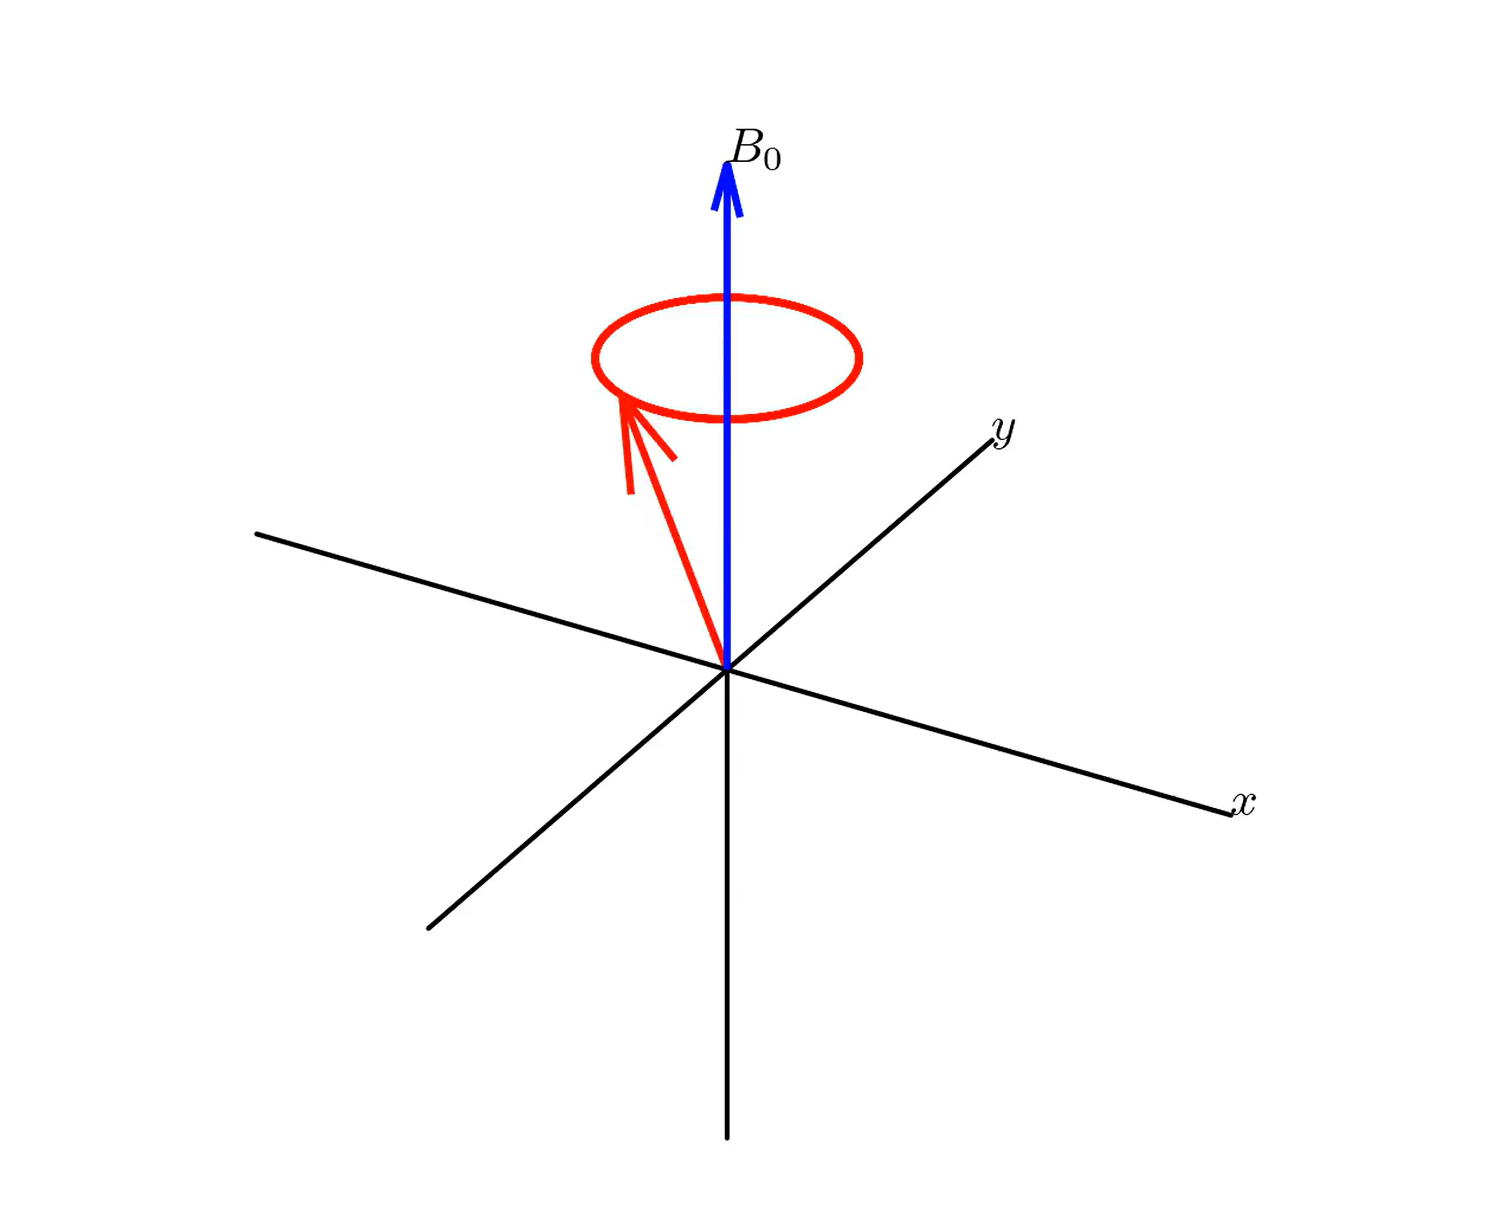
\includegraphics[width=\linewidth]{figs/larmor-precession.png}
            \caption{Larmor precession about $\Bnot$}
        \end{figure}
        
    \end{minipage}
    
\end{frame}

%------------------------------------------------
 

\begin{frame}{Net Magnetization and Relaxation}

    With many spins, any material can acquire a net magentization.

    Along $\hat{z}$, statistical mechanics tells us that 

    \begin{equation}
        \frac{N_+}{N_-} = \exp\left(\frac{\gamma \hbar B_0}{k T}\right)
    \end{equation}
    with total \textbf{net magnetization}
    \begin{equation}
        M_z = \sum_i \gamma \hbar m_i = \frac{\hbar}{2} \gamma (N_+ - N_-)
    \end{equation}
    Expect spins to eventually re-align with $\hat{z}$ direction. 
\end{frame}
%------------------------------------------------


\begin{frame}{Producing Transverse Magnetization}
    \begin{block}{Circularly Polarized Field}
        \begin{equation}
            \vec{B_1}(t) = B_1\cos(\omega_0t)\hat{x}
        \end{equation}        
    \end{block}
    To ``tip'' magnetization into $xy$ plane, apply a circularly polarized $\Bone (t)$. Classical torque result in a rotating frame yields, 

    
    \begin{equation}
        \vec{B}^* = \left(\left[\Bnot- \frac{\omega_0}{\gamma}\right] \hat{z}^* + B_1 \hat{x}^*\right)
    \end{equation}
\end{frame}

%------------------------------------------------
\begin{frame}{$\halfpi$ and $\pi$ pusles}
    \begin{figure}
        \centering
        \begin{subfigure}{0.4\linewidth}
            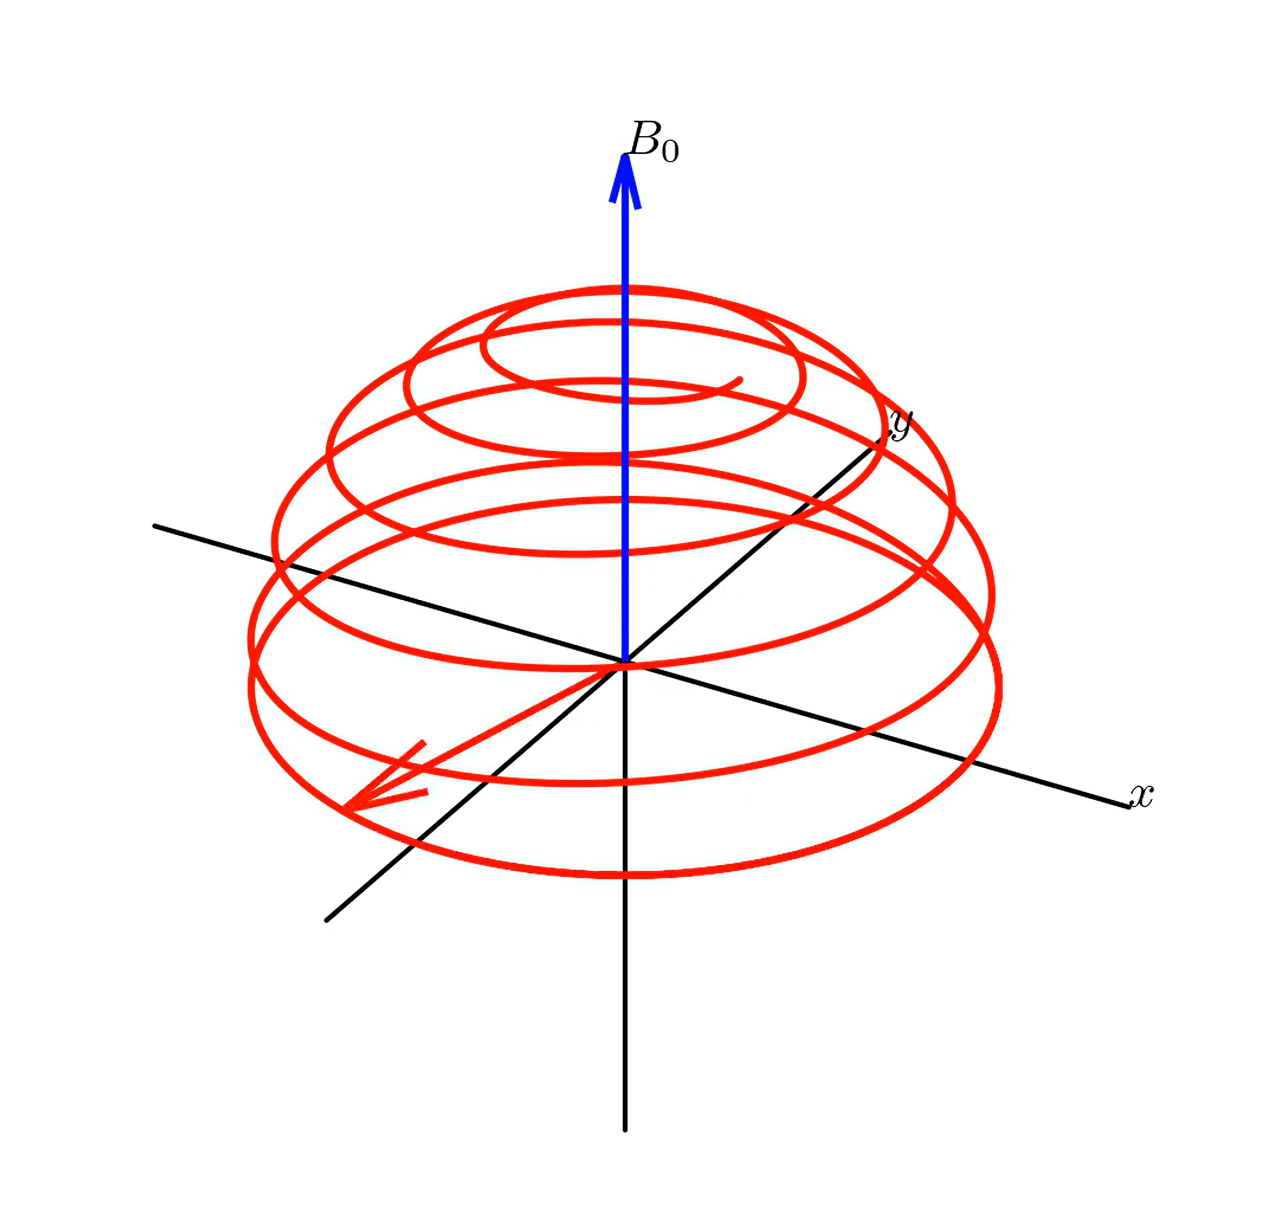
\includegraphics[width = \linewidth]{figs/pi-2-pulse.png}
            \caption{$\halfpi$ pulse produces transverse magentization}
        \end{subfigure}
        \begin{subfigure}{0.4\linewidth}
            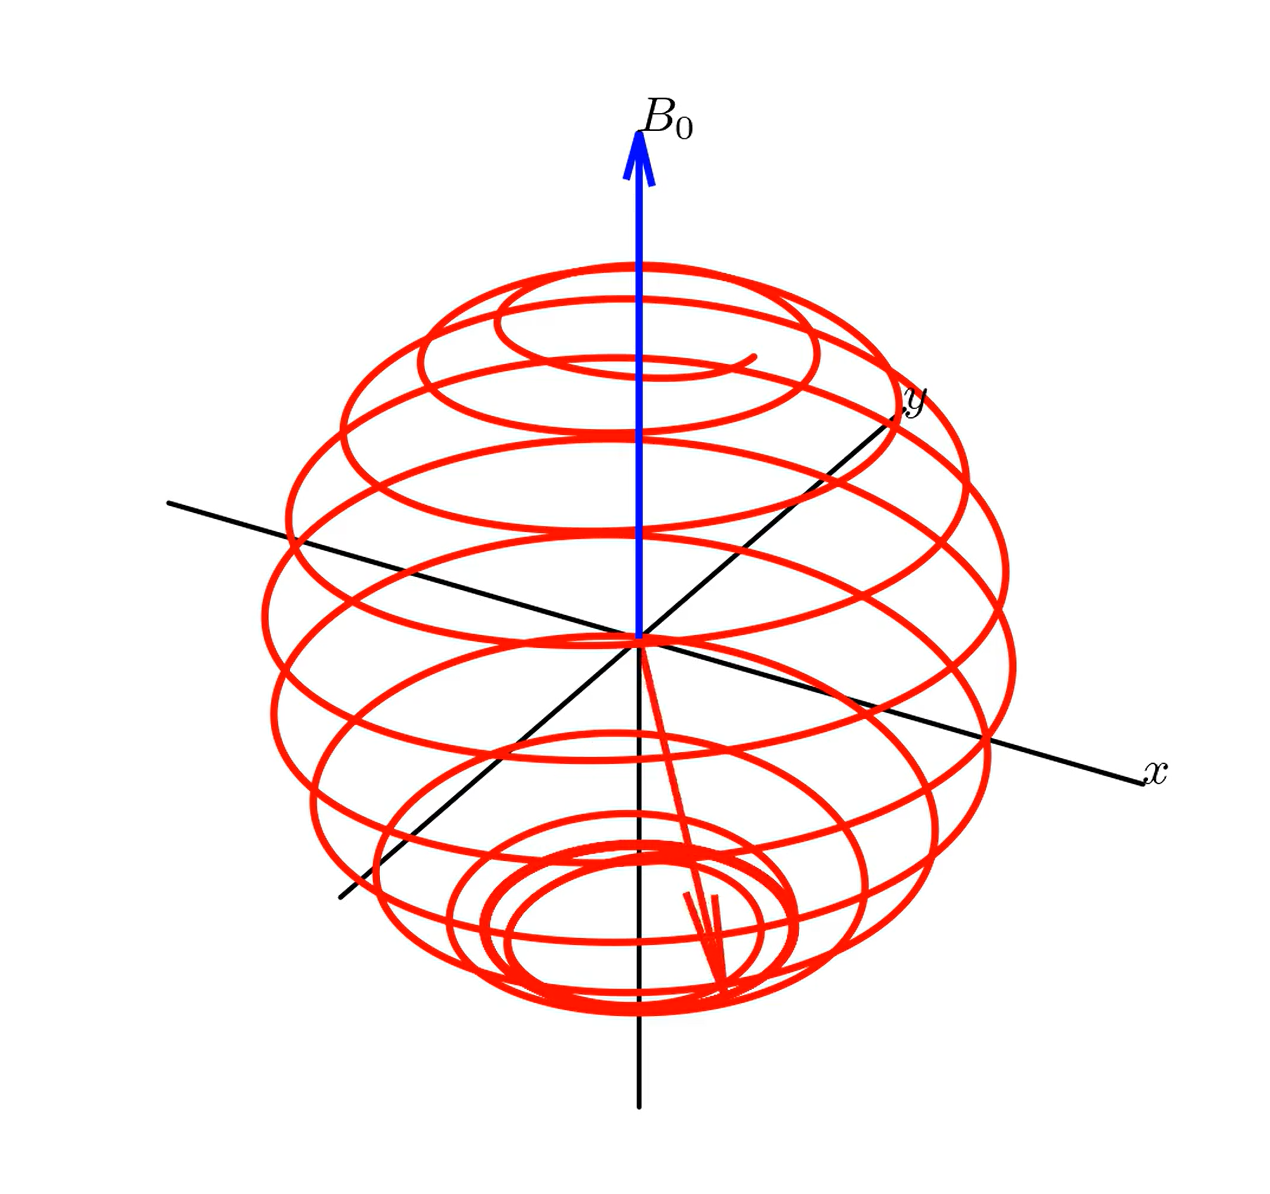
\includegraphics[width = \linewidth]{figs/pi-pulse.png}
            \caption{$\pi$ pulse flips magentization from $+\hat{z}$ to $-\hat{z}$}
        \end{subfigure}
        \caption{$\langle \vec{S} \rangle$ over time during a $\halfpi$ and $\pi$ pulse}\label{fig:pulse-spirals}
    \end{figure}
\end{frame}

\begin{frame}{Spin-Lattice Relaxation $(T_1)$}
    Time constant associated with decay of net magnetization back towards $+\hat{z}$. 

    \begin{equation}\label{eqn:bloch-t1}
        \frac{d \vec{M}(t)}{dt} = \frac{\vec{M}(t)-\vec{M_0}}{T_1}
    \end{equation}
    Referred to as the \textbf{Bloch equations}. 
\end{frame}

\begin{frame}{Spin-Spin Relaxation $(T_2)$}
    Time constant associated with the decay of the relative ``coherence'' of spins in $xy$ plane, with associated Bloch equation \cite{principles-resonance},    

    \begin{equation}\label{eqn:bloch-t2}
        \frac{d\vec{M}_{x,y}}{dt} = \frac{\vec{M}_{x,y}}{T_2}
    \end{equation}
\end{frame}

\begin{frame}{Free Induction Decay and $T_2^*$}

    \begin{minipage}{0.6\textwidth}
        \begin{itemize}
            \item Observations performed with a pickup coil detecting flux in transverse direction
            \item Magnetization becomes increasingly decoherent; produces \textbf{free induction decay (FID)} signal
            \item Combined effects of spin-lattice, spin-spin, and field inhomogeneities \cite{principles-resonance}
        \end{itemize}
        \begin{equation}
            \frac{1}{T_2^*} = \frac{1}{T_1}+\frac{1}{T_2}+ \gamma \Delta B_0
        \end{equation}
    \end{minipage}
    \hfill
    \begin{minipage}{0.3\textwidth}
        \begin{figure}
            \centering
            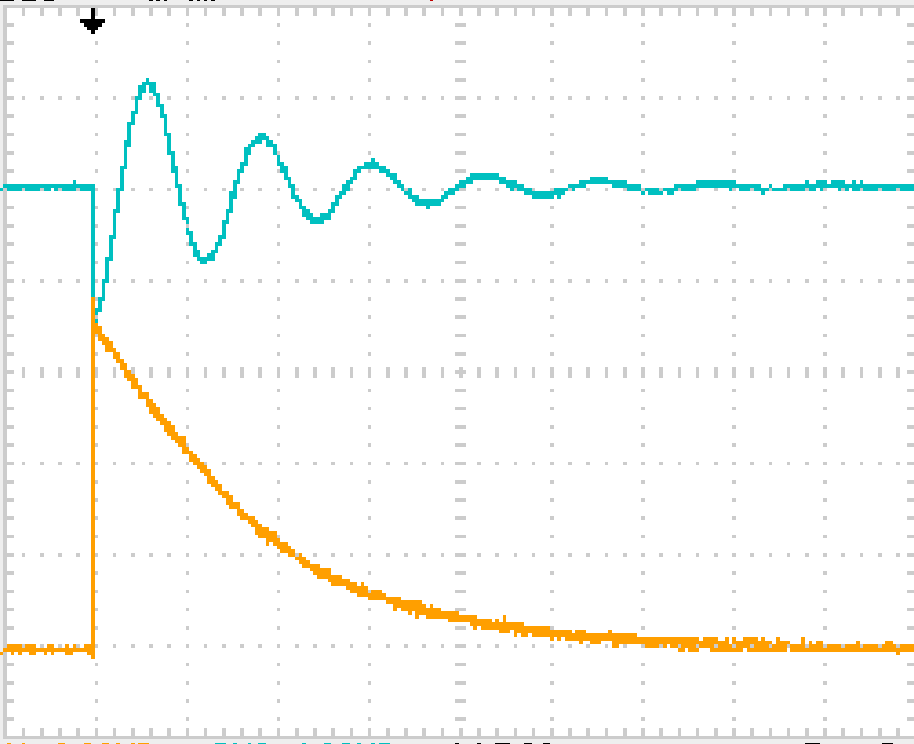
\includegraphics[width=\textwidth]{figs/basic_fid.png}
            \caption{Basic FID signal of mineral oil \cite{lab-manual}}
        \end{figure}
    \end{minipage}
    
%------------------------------------------------
\end{frame}


\section{Apparatus and Experimental Procedures}

\begin{frame}{Apparatus: TeachSpin NMR Set} 
    \begin{figure}
        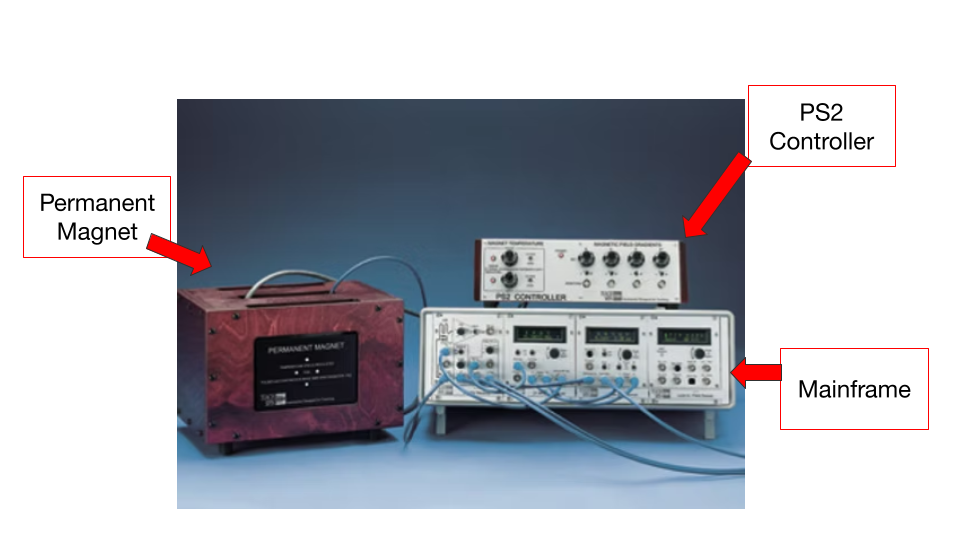
\includegraphics[width = 0.8\linewidth]{figs/teachspin.png}
        \caption{Pulsed/CW NMR Spectrometer, PS2-B}
    \end{figure}
\end{frame}

\begin{frame}{Permanent Magnet}
    \begin{itemize}
        \item .5 T magnetic field
        \item RF sample measurement coil
        \item Tuning capacitors (find resonance with RF coil)
        \item Thermal servo units/Field gradient coils 
    \end{itemize}

    \begin{figure}
        \centering
        \begin{subfigure}{0.35\linewidth}
            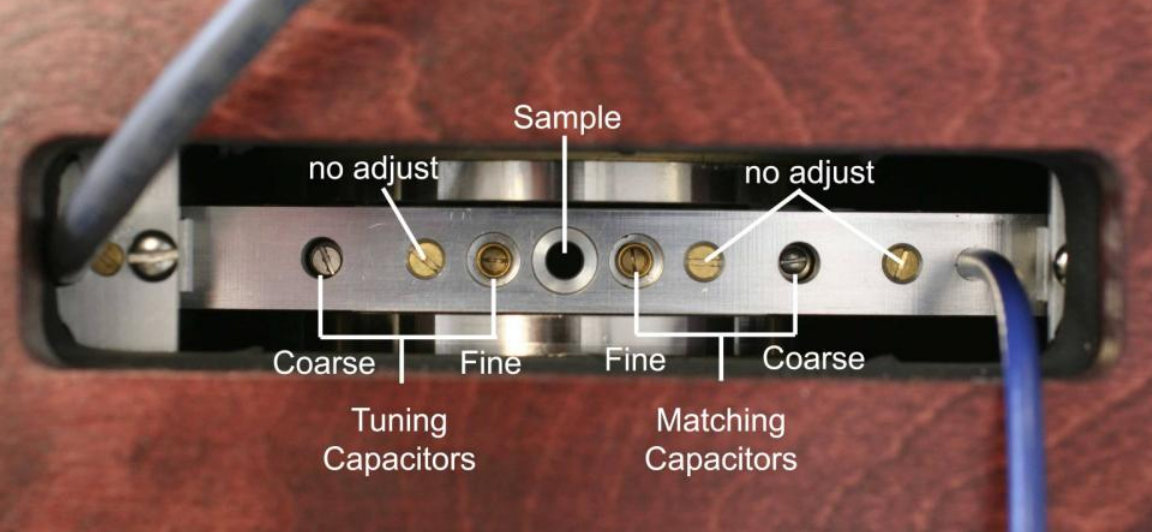
\includegraphics[width = \linewidth]{figs/above.png}
            \caption{Capacitors}
        \end{subfigure}
        \begin{subfigure}{0.3\linewidth}
            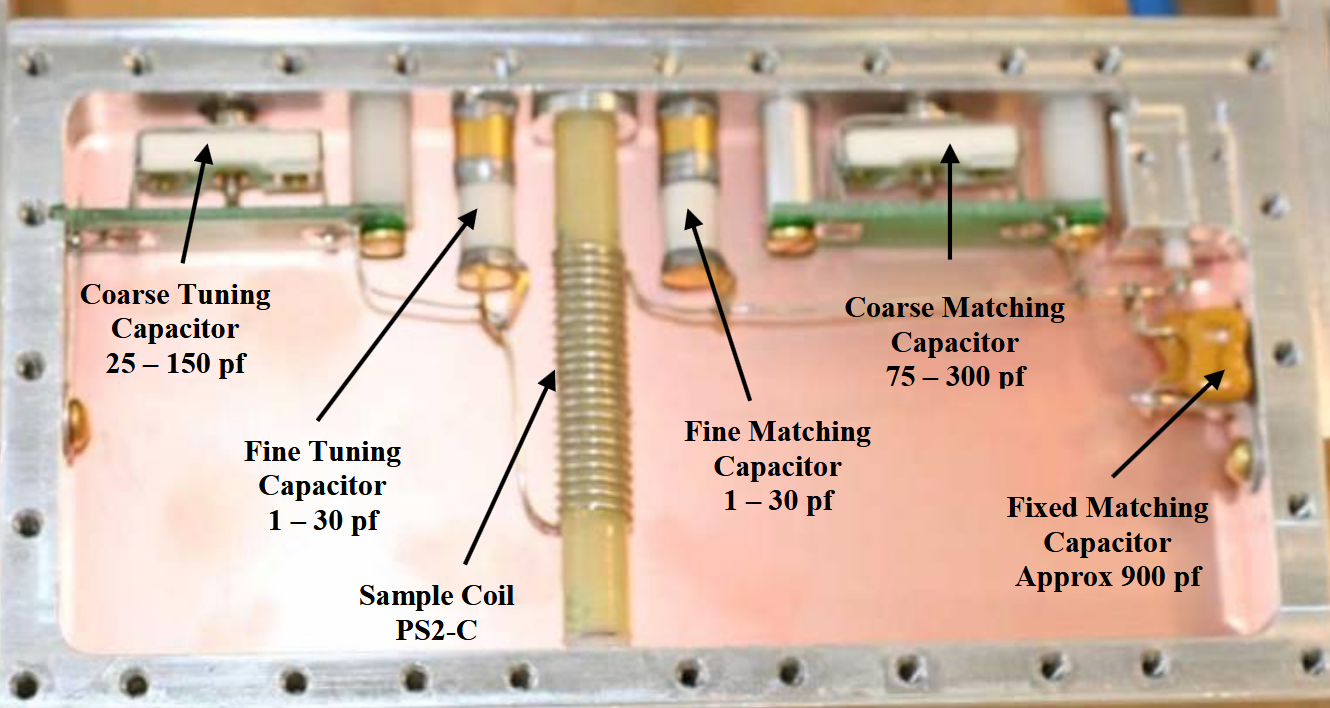
\includegraphics[width = \linewidth]{figs/coils.png}
            \caption{RF Coil}
        \end{subfigure}
        \caption{Diagrams of RF coil and capacitors}\label{fig:coils}
    \end{figure}
\end{frame}


\begin{frame}{PS2 Controller}
    \begin{itemize}
        \item Field gradient coil control $\rightarrow$ Maximize homogeneity
        \item Magnet temperature control $\rightarrow$ Indicate reference temperature 
    \end{itemize}
    \begin{figure}
        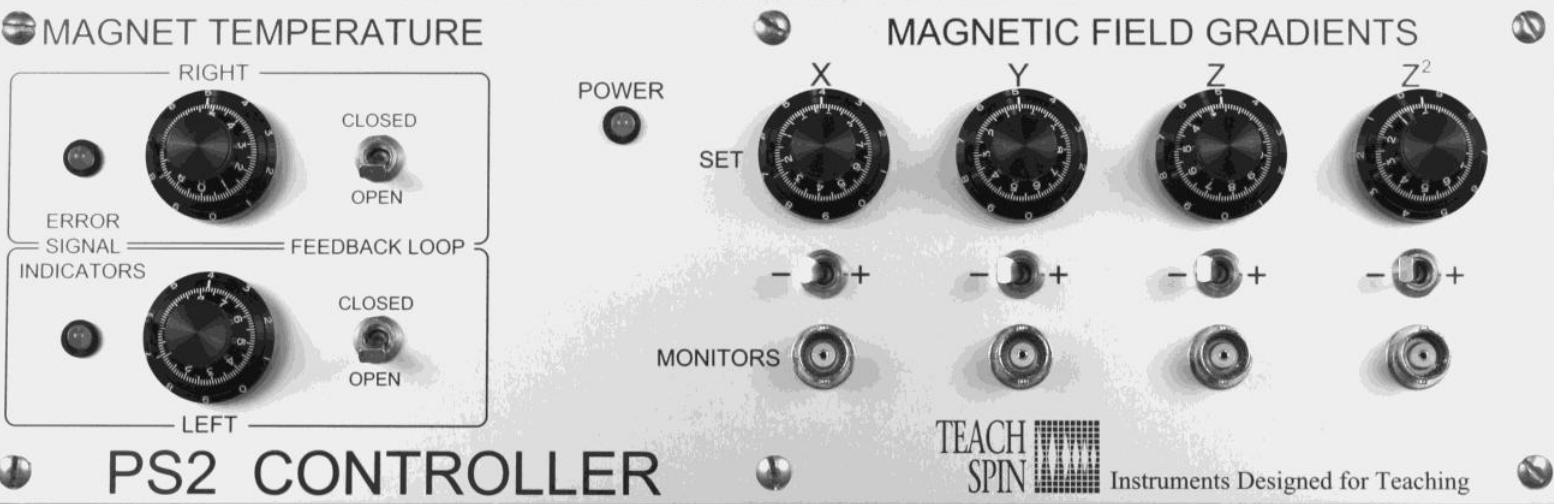
\includegraphics[width = 0.6\linewidth]{figs/temp-controller.png}
        \caption{Temperature controller}
    \end{figure}
\end{frame}

\begin{frame}{Mainframe}
    \begin{minipage}{0.4\linewidth}
        \begin{itemize}
            \item Receiver
            \begin{itemize}
                \item Process RF sample signal 
                \item Tunable gain and filter
            \end{itemize}
            \item Synthesizer
            \begin{itemize}
                \item Generates RF excitation signal 
            \end{itemize}
            \item Pulse Programmer $\rightarrow$ Some Controls: 
            \begin{itemize}
                \item A and B length
                \item A and B delay time
            \end{itemize} 
        \end{itemize}
    \end{minipage}
    \hfill
    \begin{minipage}{0.5\linewidth}
        \begin{figure}
            \centering
            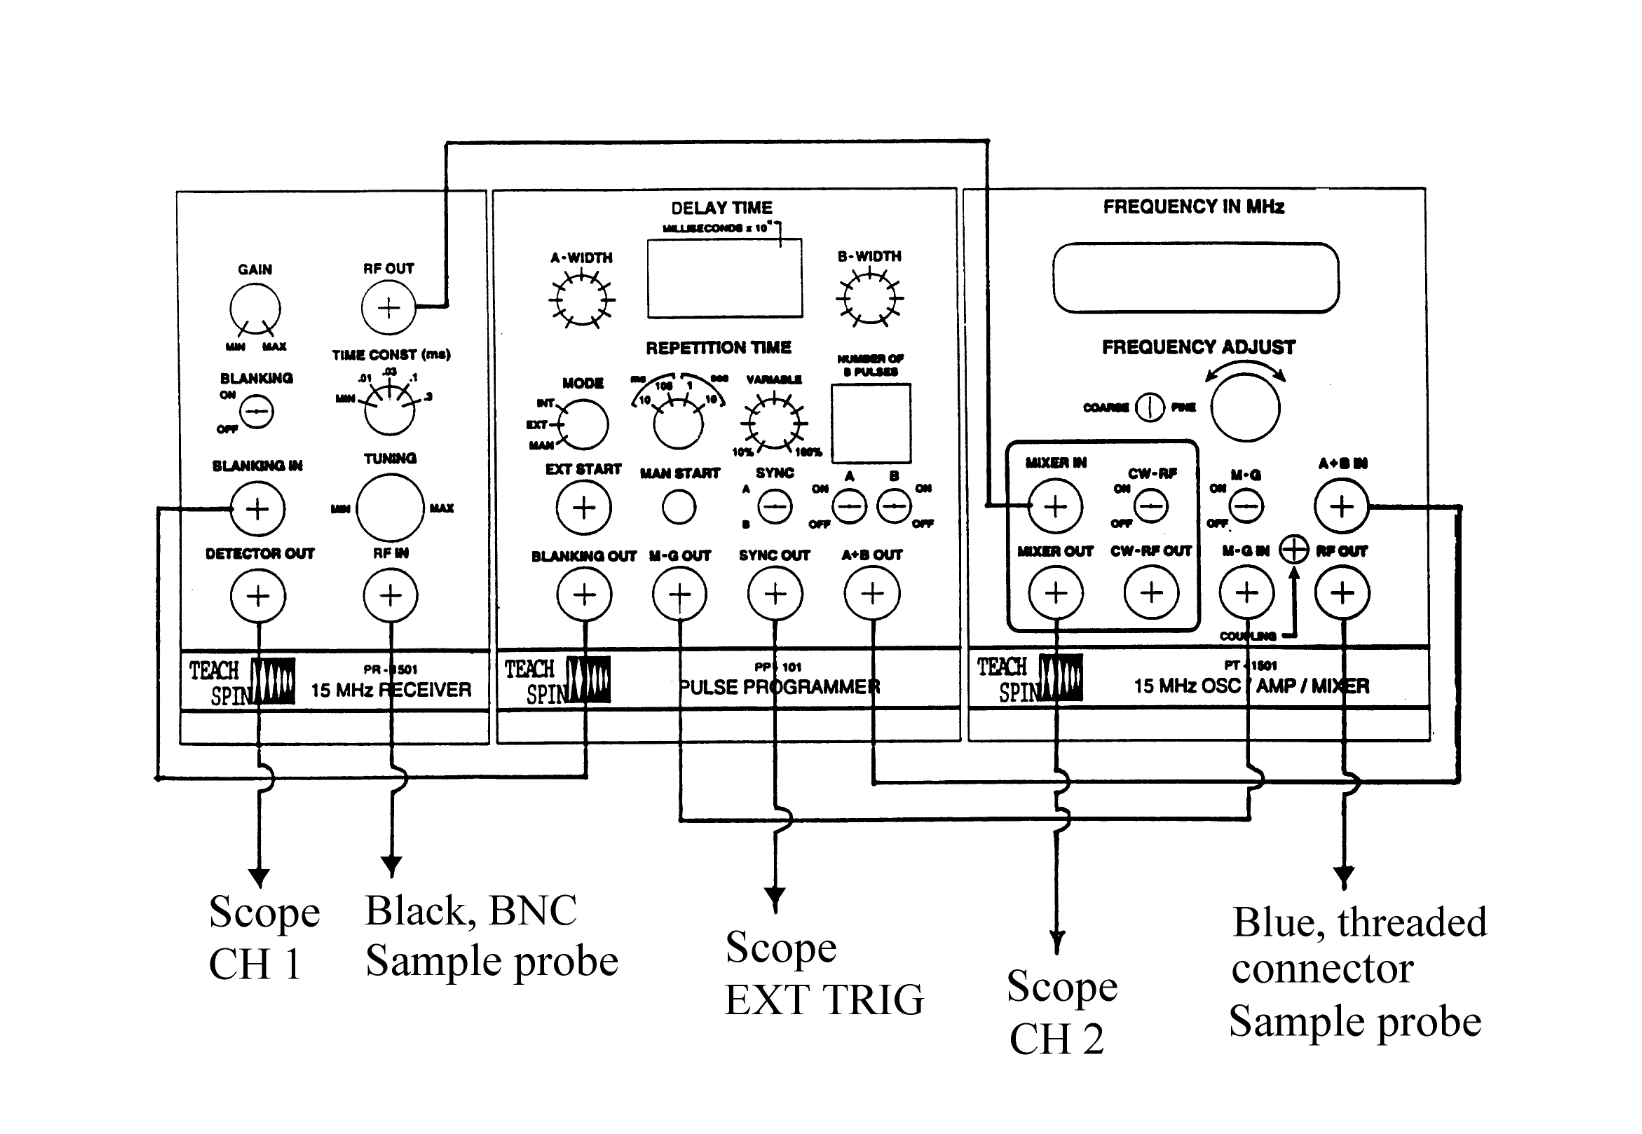
\includegraphics[width = 0.9\linewidth]{figs/mainframe.png}
            \caption{Mainframe (deprecated)}
        \end{figure}
    \end{minipage}
\end{frame}

\begin{frame}{Some Notes on Pulse Sequencing}
    Recall,
    \begin{alertblock}{$\halfpi$ pulse}
        \begin{itemize}
            \item Flips net magnetization into $xy$ plane
            \item Generates FID signal
        \end{itemize}
    \end{alertblock}

    \begin{alertblock}{$\pi$ pulse}
        \begin{itemize}
            \item Flips net magnetization along $-\hat{z}$ axis
            \item No FID signal
        \end{itemize}
    \end{alertblock}
\end{frame}

\begin{frame}{What happens after a $\halfpi$ pulse?}
    \begin{itemize}
        \item FID signal decays primarily due to spin dephasing from field inhomogeneities* 
        \item Spins decay back to the $+\hat{z}$-axis (even after FID signal disappears)
    \end{itemize}
\end{frame}

\begin{frame}{Dephasing due to field inhomogeneities}
    \begin{itemize}
        \item Static magnetic field pointing in z produces a torque that causes the spin to rotate in the $xy$ plane 
        \item Different field magnitudes cause different rotation speeds 
        \item If all the spins are aligned in the $xy$ plane, FID signal is strong
        \item If they are misaligned (out of phase), FID signal is weak
        \item This makes it hard to measure $T_2$
    \end{itemize}
\end{frame}

\begin{frame}{What happens after a $\pi$ pulse?}
    \begin{itemize}
        \item FID does not form since spins are not in $xy$ plane
        \item Spins decay back to the +z-axis (no FID signal forms) 
    \end{itemize}
\end{frame}


\begin{frame}{$T_1$ Measurement Sequence: $\halfpi - \pi$}
    \begin{itemize}
        \item Apply a $\halfpi$ pulse.
        \begin{itemize}
            \item Magnetization enters $xy$ plane and dephases
            Spins slowly decay to $+\hat{z}$
        \end{itemize}
        \item Apply another $\halfpi$ pulse a little later
        \begin{itemize}
            \item $xy$ spins kicked to the $-\hat{z}$-axis (no FID signal)
            \item $+\hat{z}$ spins kicked to the $xy$ (FID signal)
        \end{itemize}
        \item Gives an idea of how fast longitudinal spins decay
    \end{itemize}
\end{frame}

\begin{frame}{$T_1$ Measurement Sequence: $\pi-\halfpi$}
    \begin{itemize}
        \item Apply a $\pi$ pulse.
        \begin{itemize}
            \item Net magnetization jumps to $-\hat{z}$ (no signal)
            \item Spins slowly decay to $+\hat{z}$
        \end{itemize}
        \item Apply a $\halfpi$ pulse a little later
        \begin{itemize}
            \item Spins along $-\hat{z}$ are kicked to $-\hat{x}$
            \item Spins along +z are kicked to $+\hat{x}$
            \item If no FID signal is produced (half life)
        \end{itemize}
        \item Much more elegant
    \end{itemize}

\end{frame}


\begin{frame}{$T_2$ Measurement Sequence: $\halfpi-\pi$}
    \begin{itemize}
        \item Apply a $\halfpi$ pulse $\rightarrow$ Net magnetization enters the $xy$ plane and dephases 
        \item Apply a $\pi$ pulse a little later
            \begin{itemize}
                \item Spins remain in $xy$ plane, but `reverse' rotation direction
                \item Spins rephase a little later 
            \end{itemize}
        \item The decay in rephasing signal follows $T_2$
    \end{itemize}
\end{frame}

\begin{frame}{Using More Pulses}
    \begin{itemize}
        \item To better characterize the decay multiple $\pi$ pulses are applied
        \item Must be close together to mitigate molecular diffusion
        \begin{itemize}
            \item Spin dephases at one speed and returns at another 
            \item Will not rephase with the rest
        \end{itemize}
    \end{itemize}
\end{frame}

\begin{frame}{Experimental Procedure: Resonance}
    \begin{itemize}
        \item Tune RF frequency to proton resonance (~21 MHz) $\rightarrow$ Minimize beats
        \item Use tuning capacitor to maximize FID signal
    \end{itemize}
\end{frame}

\begin{frame}{$\halfpi$ and $\pi$ pulses}
    \begin{itemize}
        \item Apply a single RF pulse and vary its length
        \item Find the length with maximum FID signal
        \item This is a $\halfpi$ pulse
        \item Double the length to find $\pi$ pulse length
    \end{itemize}
\end{frame}

\begin{frame}{Sequencing}
    \begin{itemize}
        \item Use adequate pulse sequences to measure decay times
        \item Record data for processing to calculate characteristic times $T_1$ and $T_2$
    \end{itemize}
\end{frame}

% FAILED ATTEMPT AT ANIMATION - WILL REMOVE LATER 
% %------------------------------------------------
% \begin{frame}{$\halfpi$ and $\pi$ pusles animated?}
%     \begin{figure}
%         \centering
%         \begin{subfigure}{0.4\linewidth}
%             \animategraphics[loop, width = \linewidth]{10}{figs/gif_attempt/pi_2_pulse/pi_2_pulse_2-}{0}{99}
%             \caption{$\halfpi$ pulse produces transverse magentization}
%         \end{subfigure}
%         \begin{subfigure}{0.4\linewidth}
%             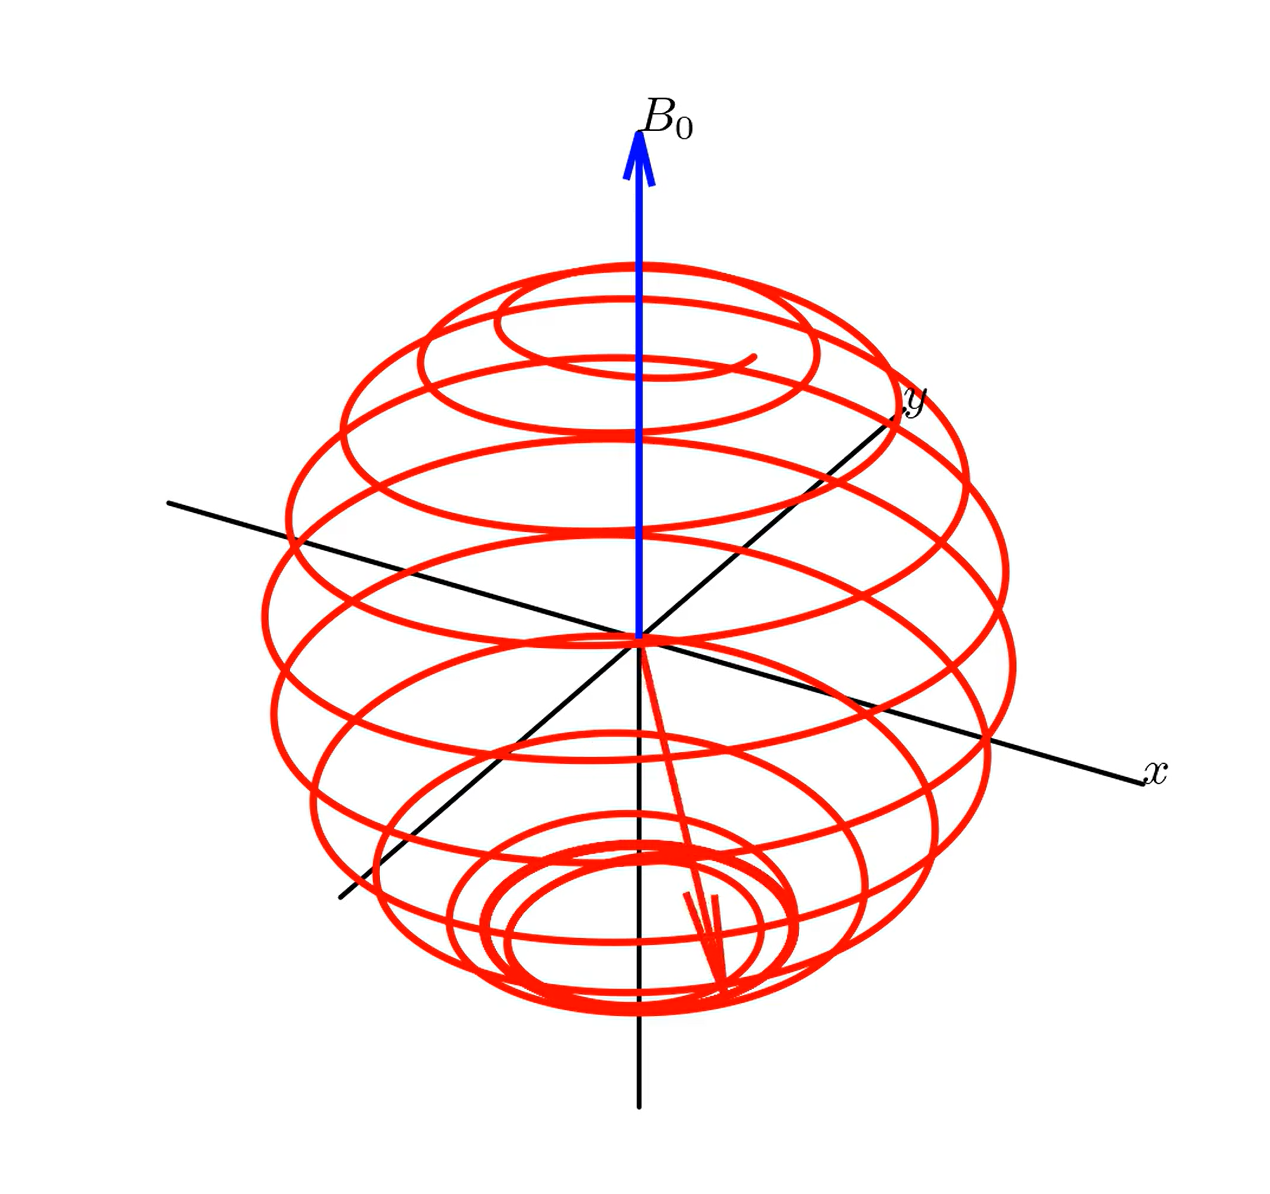
\includegraphics[width = \linewidth]{figs/pi-pulse.png}
%             \caption{$\pi$ pulse flips magentization from $+\hat{z}$ to $-\hat{z}$}
%         \end{subfigure}
%         \caption{$\langle \vec{S} \rangle$ over time during a $\halfpi$ and $\pi$ pulse}\label{fig:pulse-spirals}
%     \end{figure}
    
% \end{frame}



%------------------------------------------------




% \begin{frame}{Blocks of Highlighted Text}
%     In this slide, some important text will be \alert{highlighted} because it's important. Please, don't abuse it.

%     \begin{block}{Block}
%         Sample text
%     \end{block}

%     \begin{alertblock}{Alertblock}
%         Sample text in red box
%     \end{alertblock}

%     \begin{examples}
%         Sample text in green box. The title of the block is ``Examples".
%     \end{examples}
% \end{frame}

% %------------------------------------------------

% \begin{frame}{Multiple Columns}
%     \begin{columns}[c] % The "c" option specifies centered vertical alignment while the "t" option is used for top vertical alignment

%         \column{.45\textwidth} % Left column and width
%         \textbf{Heading}
%         \begin{enumerate}
%             \item Statement
%             \item Explanation
%             \item Example
%         \end{enumerate}

%         \column{.45\textwidth} % Right column and width
%         Lorem ipsum dolor sit amet, consectetur adipiscing elit. Integer lectus nisl, ultricies in feugiat rutrum, porttitor sit amet augue. Aliquam ut tortor mauris. Sed volutpat ante purus, quis accumsan dolor.

%     \end{columns}
% \end{frame}

% %------------------------------------------------
% \section{Second Section}
% %------------------------------------------------

% \begin{frame}{Table}
%     \begin{table}
%         \begin{tabular}{l l l}
%             \toprule
%             \textbf{Treatments} & \textbf{Response 1} & \textbf{Response 2} \\
%             \midrule
%             Treatment 1         & 0.0003262           & 0.562               \\
%             Treatment 2         & 0.0015681           & 0.910               \\
%             Treatment 3         & 0.0009271           & 0.296               \\
%             \bottomrule
%         \end{tabular}
%         \caption{Table caption}
%     \end{table}
% \end{frame}

% %------------------------------------------------

% \begin{frame}{Theorem}
%     \begin{theorem}[Mass--energy equivalence]
%         $E = mc^2$
%     \end{theorem}
% \end{frame}

% %------------------------------------------------

% \begin{frame}{Figure}
%     Uncomment the code on this slide to include your own image from the same directory as the template .TeX file.
%     %\begin{figure}
%     %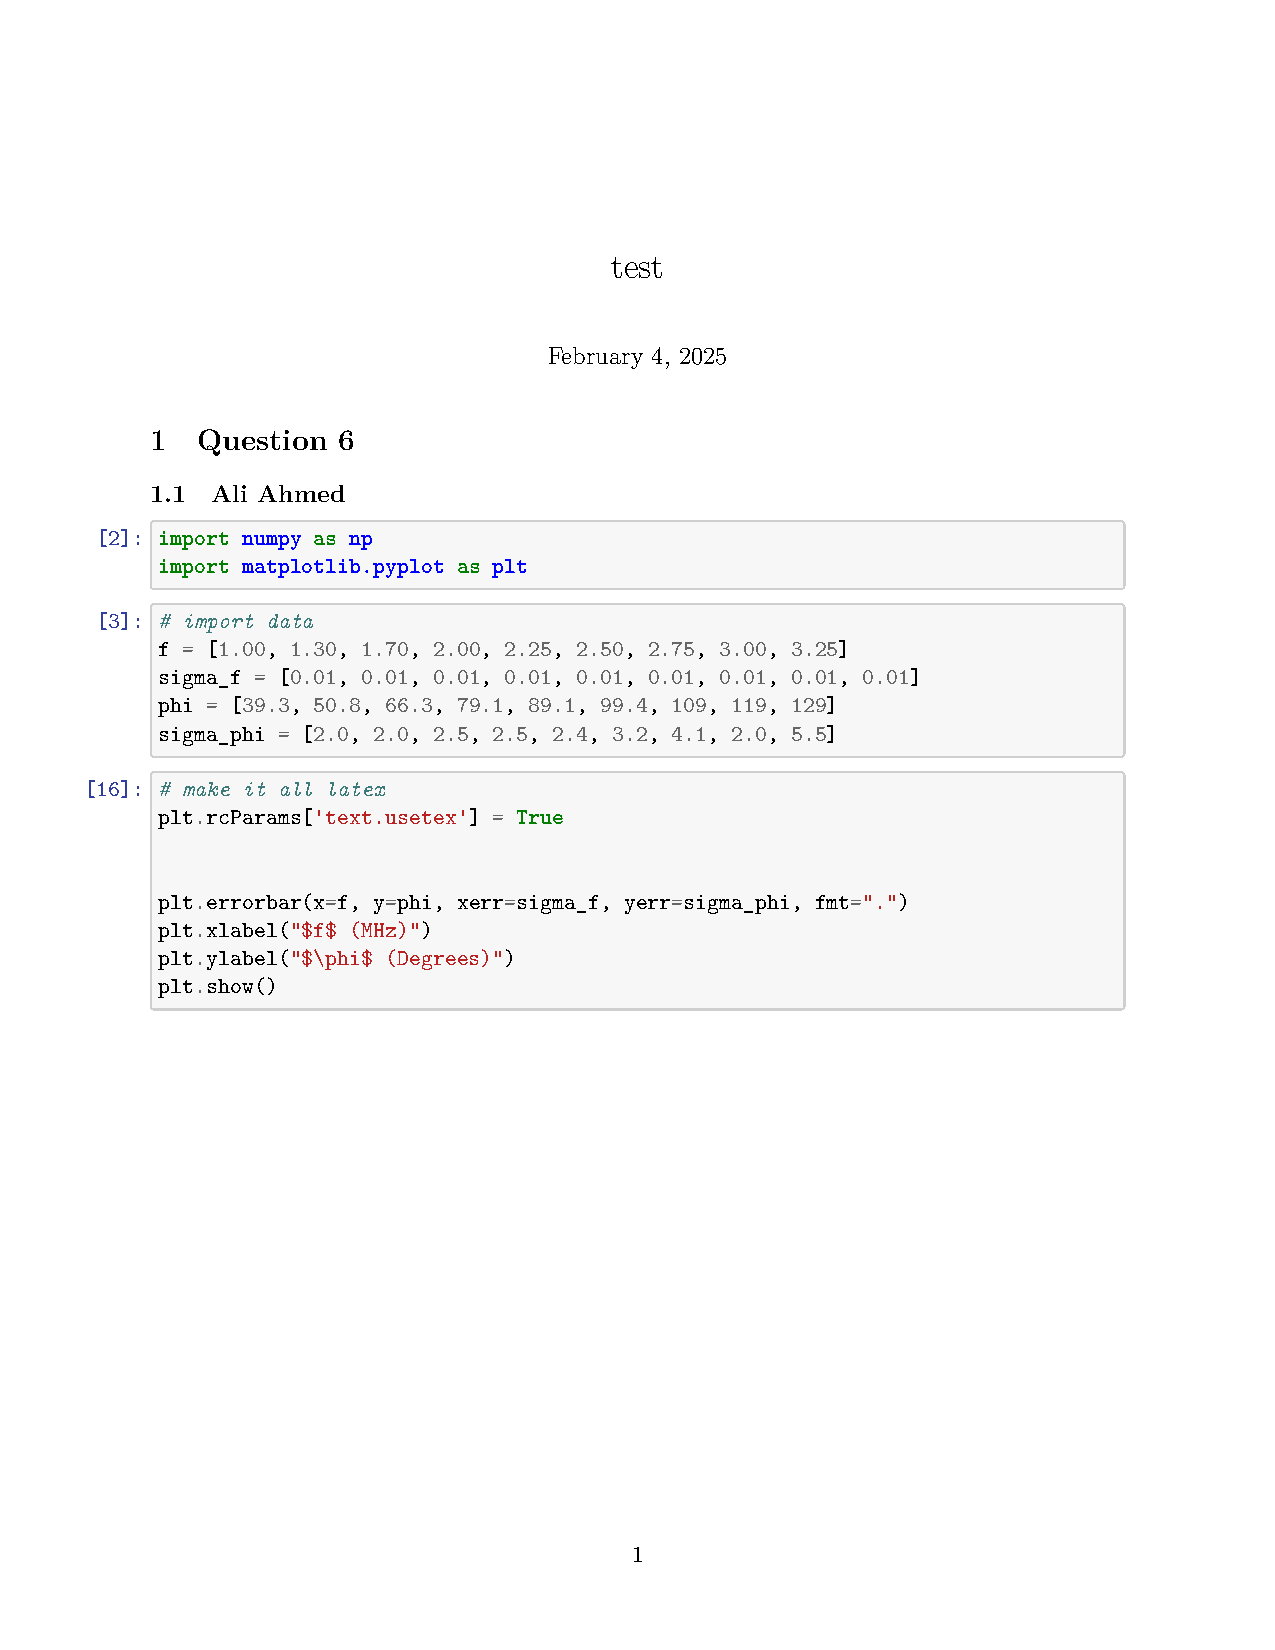
\includegraphics[width=0.8\linewidth]{test}
%     %\end{figure}
% \end{frame}

% %------------------------------------------------

% \begin{frame}[fragile] % Need to use the fragile option when verbatim is used in the slide
%     \frametitle{Citation}
%     An example of the \verb|\cite| command to cite within the presentation:\\~

%     This statement requires citation \cite{p1}.
% \end{frame}

% %------------------------------------------------

\begin{frame}{References}
    \footnotesize
    \bibliographystyle{ieeetr}
    \bibliography{reference.bib}

\end{frame}

% %------------------------------------------------

% \begin{frame}
%     \Huge{\centerline{\textbf{The End}}}
% \end{frame}

%----------------------------------------------------------------------------------------

\end{document}